%% File 'sample.tex'
%% 
%% Copyright (C) 2003 by Maarten Sneep <sneep@nat.vu.nl>
%% Modified 2004 by B.Ph. van Milligen <boudewijn.vanmilligen@ciemat.es>
%% 
%% This file may be distributed and/or modified under the conditions of
%% the LaTeX Project Public License, either version 1.2 of this license
%% or (at your option) any later version.  The latest version of this
%% license is in:
%% 
%%    http://www.latex-project.org/lppl.txt
%% 
%% and version 1.2 or later is part of all distributions of LaTeX version
%% 1999/12/01 or later.
%% 
\documentclass{epsconf}
\usepackage{graphicx}
%\usepackage{epsfig} % use this package to include EPS format figures
\usepackage{wrapfig}
\usepackage{amsmath}
\usepackage{amssymb}
\newcommand{\bb}[1]{\textbf{#1}}

\title{Dependence of the Nonhelical Dynamo on Shear: Numerical Exploration of the Magnetic Shear-current and Stochastic-$\alpha$ Effects}
\author{\underline{A. Hankla}$^1$, C. Fendt$^1$}
\institute{$^1$ Max Planck Institute for Astronomy, Heidelberg, Germany}

\begin{document}
\maketitle

\section{Introduction}
Accretion disks are ubiquitous in astrophysical systems, ranging in scales from propoplanetary disks around stars to disks around active galactic nuclei (AGN). When the disk is mostly ionized and threaded by a weak magnetic field, the magnetorotational instability (MRI) leads to radially-inward transport of angular momentum and hence accretion. At its heart, the MRI is a shear-driven instability: the importance of shear was therefore explored early on, exposing numerical and analytical evidence for how various quantities scale~\cite{abl96}.\\
%
However, some of these previous works may have cut out important physics due to numerical constraints that limit the simulation regime. Indeed, Ref.~\cite{SSH16} finds that within the shearing box framework, used by all of the above papers, the vertical height of the simulation domain is particularly important so as not to artificially dampen a large-scale dynamo. In exploring the aforementioned scalings as well as some others over a broad range of shearing parameter in a large unstratified box, we uncover an abrupt (previously unreported) jump as a function of shear that we suspect to be connected to the presence/absence of a large-scale dynamo. \\
%
We study unstratified systems, whose additional reflectional symmetry means that the dynamo presence cannot by explained by the well-known $\alpha$-effect. Instead we investigate two rival models: the magnetic shear-current effect, proposed by Ref.~\cite{SB16} as an analog to the kinematic shear-current effect fueled by a negative off-diagonal diffusivity, and the stochastic $\alpha$ effect, motivated by fluctuations in the $\alpha$ dynamo parameter that average to zero over many physical realizations~\cite{hms11}. Comparison of these two models is facilitated by explicitly calculating transport coefficients and adjusting the simulation domain size XX. We note that, unlike for the so-called ``butterfly diagrams" of $\alpha\Omega$ dynamos~\cite{GP15}, there is currently no analytic reasoning behind the cycles of the mean azimuthal magnetic field, for an unstratified dynamo: we therefore provide preliminary scalings to motivate future analytic research. \\
%
Although accretion disks are in general vertically stratified, the midplane region of the disk is roughly unstratified. Therefore we can compare our results to the inner portion of previous studies' stratified shearing boxes. Unstratified shearing boxes also provide a clean environment to explore these dynamo mechanisms without fear of pollution by the $\alpha$ effect.

\section{Methods} \label{sec:methods}
%\subsection{Equations solved and code description}
The basis of this project is solving the ideal compressible single-fluid magnetohydrodynamic (MHD) equations within the unstratified shearing box approximation. This is done by using the $\texttt{ATHENA}$ code with the CTU integrator, Roe Riemann solver, and the FARGO orbital advection scheme~\cite{StoneGardiner2010}. The equations solved are as follows:
\begin{align}
    \frac{\partial\rho}{\partial t}+\nabla\cdot(\rho\bb{v})=0, &\hspace{.5in}  \frac{\partial\bb{B}}{\partial t} - \nabla\times(\bb{v}\times\bb{B})=0, \\
    \frac{\partial\rho\bb{v}}{\partial t} + \nabla\cdot(\rho\bb{vv}+\bb{T})&= -2\rho\Omega\hat z\times\bb{v}+2q\rho\Omega^2~x\hat x
\end{align}
where 
\begin{equation*}
    \bb{T} = \left(P+\frac{\bb{B}\cdot\bb{B}}{8\pi}\right)\bb{I}-\frac{\bb{BB}}{4\pi}
\end{equation*}
is the total stress tensor. As usual, $\rho$ is mass density, $\bb{v}$ is the plasma velocity, and $\bb{B}$ is the magnetic field. Here, the disk is rotating with angular frequency $\Omega\hat z$, and $\hat x$ is the radial direction. The main focus of this work varies the shearing parameter $q$, defined through $\Omega\sim r^{-q}$ as $q=-d\ln\Omega/d\ln r$. Hence $q=3/2$ corresponds to the familiar Keplerian rotation profile.\\
%
Simulations are run with an adiabatic equation of state with a box size of $[L_x,~L_y,~L_z] = [1,~4,~4] H$ and resolution of 64, 128, and 256 zones, or 64, 32, and 64 zones/$H$, unless otherwise stated. The magnetic field configuration is $\bb{B}=B_0\sin(2\pi x/L_x)\hat z$ (zero net flux) with $B_0$ defined via the plasma beta parameter $\beta = 8\pi P_0/B_0^2 = 4000$. \\
%
%\subsection{Calculation of Transport Coefficients: Projection Method}
To make contact with the magnetic shear-current model, we calculate the transport coefficients that appear out of dynamo mean field theory: after assuming scale separation between the large-scale mean field and the small-scale turbulent field $\mathbf{B_T}=\bar{\bb{B}}+\bb{b}$ where the volume average (denoted by $\langle\cdot\rangle$) of the turbulent field $\langle\bb{b}\rangle=0$, the mean field portion of the induction equation becomes
\begin{align*}
    \frac{\partial\bar{\bb{B}}(z)}{\partial t}&=\nabla\times\left(\bb{v}(z)\times\bar{\bb{B}}(z)+\mathcal{E}(z)-(q\Omega x\hat y)\times\bar{\bb{B}}(z)\right)
\end{align*}
where $\mathcal{E}=\langle \bb{v}\times\bb{b}\rangle$ is the mean electromotive force. Scale-separation arguments yield
\begin{equation*}
    \mathcal{E}_i = \alpha_{ij}\bar{B}_j-\eta_{ij}(\nabla\times\bar{B})_j
\end{equation*}
where we have used that $B_z = 0$ and that the mean fields depend only on the $z$-direction. To directly calculate the dynamo transport coefficients $\alpha$ and $\eta$, we employ the projection method outlined in Ref.~\cite{SB16}. We calculate $\mathcal{E}$, $\bar{\bb{B}}$, and $\partial_i\bar{\bb{B}}$ from simulation data, compute $\langle\mathcal{E}_iM\rangle$ for each $M=(\bar B_x, \bar B_y, \partial_z\bar B_x, \partial_z\bar B_y)$, and solve using least-squares regression methods at each time step. We impose the constraints $\alpha_{xx}=\alpha_{yy}$, $\alpha_{yx}=0=\eta_{xy}$, and $\eta_{xx}=\eta_{yy}$ for cleaner results~\cite{SB16}. \\

\section{Results}
\begin{wrapfigure}{r}{0.6\textwidth}
\vspace{-1cm} \begin{center}
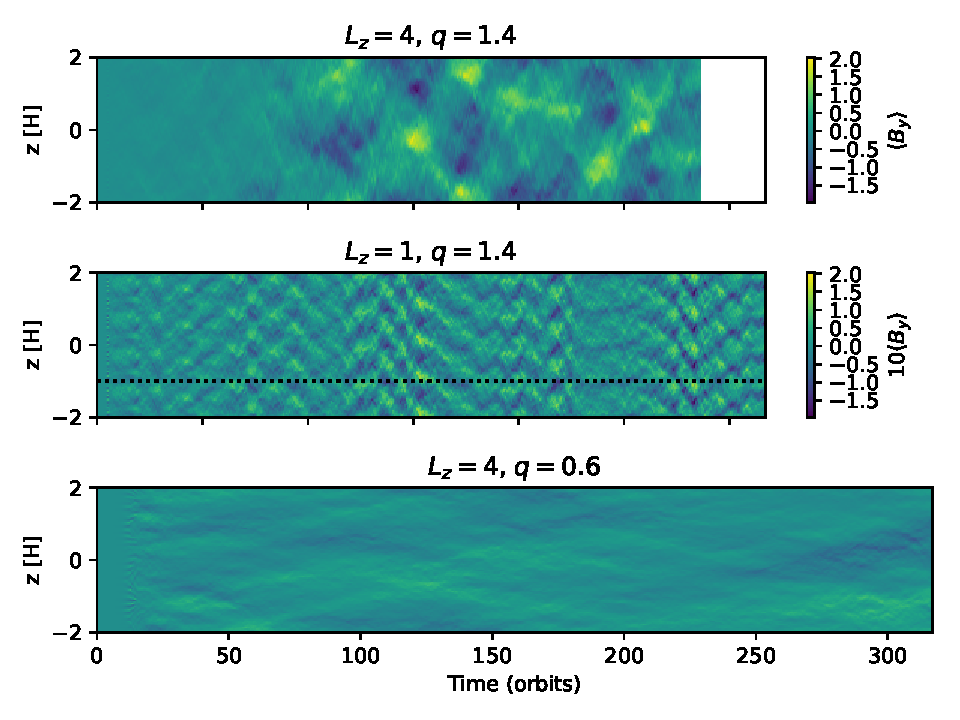
\includegraphics[width=\linewidth]{fig_xyazte_butterfly_compare_qz.pdf}
\caption{\it \small The small box has been duplicated 4 times to have the same aspect ratio. Dotted black line shows the actual simulated domain. Color bar is the same for middle and bottom.}
\label{fig:butterfly}
\end{center} 
\vspace{-1cm}
\end{wrapfigure}%
We first seek to show that a large-scale dynamo is indeed present. Convincing evidence for a large-scale magnetic field comes from the butterfly diagrams, that is, the mean azimuthal magnetic field as a function of height and time. We compare a small box, a tall box with $q>1.2$, and a tall box with $q<1.2$ in Fig.~\ref{fig:butterfly}. The tall box with dynamo action has patches of magnetic field that are on the order of $H$, whereas the small box/low $q$ do not.\\
%
Dynamo action also manifests in volume-averaged quantities such as the ratio of mean to turbulent magnetic field energy in Figure~\ref{fig:mtbr}. For small values of $q$, the mean energy is only about one-fifth of the turbulent field energy, whereas for $q\gtrapprox1.2$ the mean and turbulent fields contribute approximately equally to the total mean energy, indicating the presence of a dynamo.%
\begin{figure}[h]
\vspace{0cm}
\begin{minipage}{0.48\textwidth}
    \centering
    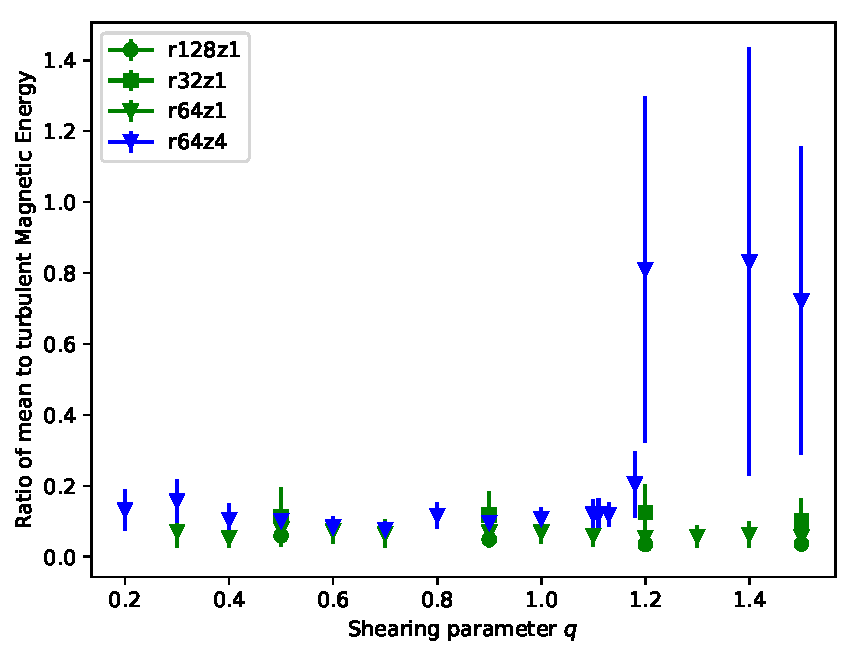
\includegraphics[width=\linewidth]{fig_vata_mtT_MEmtr_err.pdf}
    \caption{\it \small Runs with varying resolution (denoted by $r$: $r32$ corresponds to 32 zones/$H$) and box height ($z1$ being $L_z=1$).}
    \label{fig:mtbr}
\end{minipage}%
\hfill%
 \begin{minipage}{.48\textwidth}
  \centering
    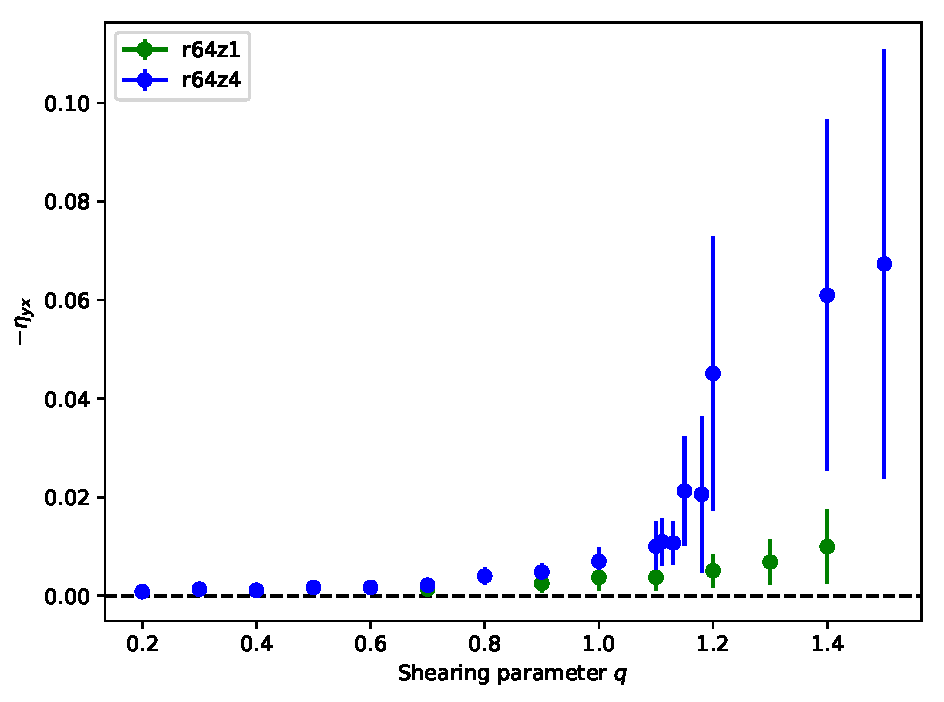
\includegraphics[width=\linewidth]{fig_vataqe_etayx_const_t100-endhgbLAIF.pdf}
    \caption{\it \small Averaged over $t=100-200$ orbits, the saturation period. Black dotted line is at zero. Error bars indicate one standard deviation. }
    \label{fig:etayx}
\end{minipage}
\vspace{0cm}
\end{figure}
%
\begin{wrapfigure}{l}{0.48\textwidth}
\begin{center} \vspace{0cm}
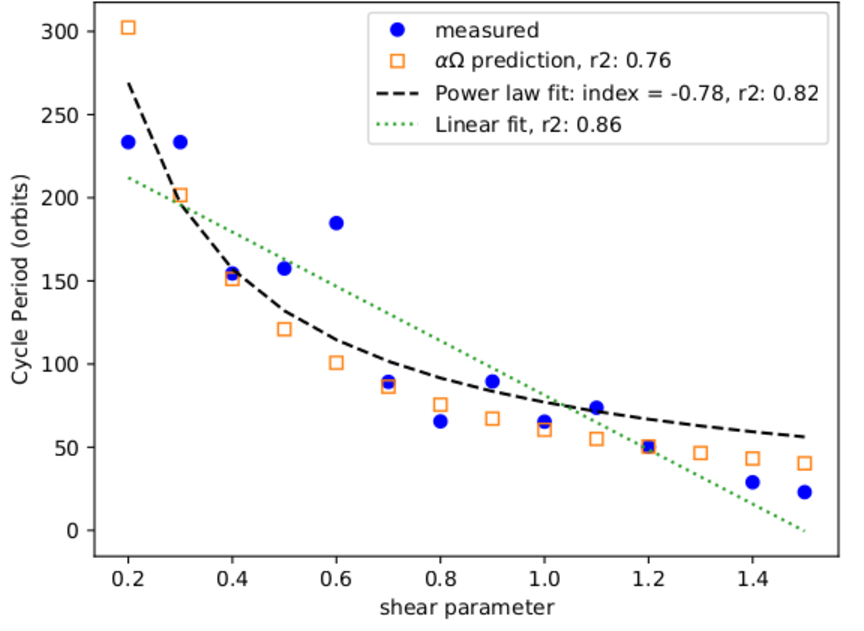
\includegraphics[width=\linewidth]{fig_q_cycle_period_hgbLAIF_r64z4b4000znf.pdf}
\caption{\it \small Comparison of $\alpha\Omega$ scaling relation period $T\sim 1/q$ and linear and power-law fits~\cite{GP15}.}
\label{fig:qperiod}
\vspace{0cm}
\end{center}
\end{wrapfigure}%
To investigate whether this break is related to a potential dynamo mechanism, we calculate the transport coefficients via the projection method (see Methods) as a function of shear. We are particularly interested in the off-diagonal component $\eta_{yx}$, which when negative supports the presence of the magnetic shear-current effect. Indeed, as seen in Fig.~\ref{fig:etayx}, this coefficient is negative for all simulations, abruptly jumps at the same $q\gtrapprox1.2$, and has the same behavior with box size as the volume-averaged quantities discussed earlier. As a check, the $\alpha$ coefficients do indeed average to zero. Ref.~\cite{LesurOgilvie08}'s toy model of a sign change in $\eta_{yx}$ due to the azimuthal magnetic field reaching a critical value is not supported because the coefficient is negative throughout the simulations. Therefore, we present in Fig.~\ref{fig:qperiod} the periods of the azimuthal field cycles as calculated from fitting the largest vertical mode's power spectrum density at a given $z$ (as in Ref.~\cite{SSH16}).  \\
%
The stochastic-$\alpha$ effect manifests through a change in dynamo growth rate when the horizontal domain size is changed. We find XXX

\section{Conclusions}
Although there is much left to consider (for instance, the effect of explicit dissipation) and much that could be improved (for instance: clearer trends appear in boxes with $L_z\approx8$, a statistical ensemble approach is the only way to rule out the stochastic-$\alpha$ effect), we have presented preliminary evidence for the presence of the magnetic shear-current effect in large, unstratified shearing boxes. 
\section{Acknowledgments}
This project was supported through a Fulbright grant of the German-American Fulbright Commission. AH is also grateful for support from the MPI Astronomy.

\begin{thebibliography}{99}
\bibitem{abl96}
M. Abramowicz, A. Brandenburg, J.-P. Lasota, MNRAS {\bf 281} (1996)
\bibitem{SSH16}
J.-M. Shi, J. Stone, and C. Huang, MNRAS {\bf 456} (2016)
\bibitem{SB16}
J. Squire and A. Bhattacharjee, J. Plasma Phys. {\bf 82} (2016)
\bibitem{hms11}
T. Heinemann, J. McWilliams, and A. Schekochihin, PRL {\bf 107} (2011)
\bibitem{GP15}
O. Gressel and M. Pessah, ApJ {\bf 810}:59, (2015)
\bibitem{StoneGardiner2010}
J. Stone and T. Gardiner, ApJ SS {\bf 189} (2010)
\bibitem{LesurOgilvie08}
G. Lesur and G. Ogilvie, A\&A {\bf 488} (2008)
\end{thebibliography}

\end{document}
\endinput
%%
%% End of file `sample.tex'.
